\documentclass{article}
\usepackage{natbib}
\usepackage{graphicx}
\usepackage[english]{babel}
\usepackage[utf8]{inputenc}
\usepackage{url}
\usepackage{fancyhdr}
\pagestyle{fancy}
\fancyhf{}
\rhead{CSI5155-Machine Learning}
\lhead{University of Ottawa}
\rfoot{Page \thepage}

\begin{document}

\begin{center}
    \textbf{\huge{CSI\_5155\_Homework\_2}}
\end{center}

\textbf{Student Name: Lingfeng Zhang}

\textbf{Student Number: 300134245}

In this homework, I used scikit-learn to analyze data.

\begin{itemize}

\item dataset preprocessing

\begin{itemize}
    \item Converting original dataset to pandas.DataFrame format to analyze.
    \item Encoding categorical features into numbers by using LabelEncoder
    \item For dataset Congressional+Voting+Records and Labor+Relations, missing values occur. Missing value imputation is applied in this dataset. SimpleInputer in scikit-learn is a simple method to impute missing values. Missing values are inputted by the most frequent category. 
\end{itemize}

\item Classifier usage and hyper-parameters

\begin{itemize}
    \item Decision Tree: sklearn.tree.DecisionTreeClassifier()
    \item Rule-based: There is no rule-based classifier in scikit-learn, so Orange.classification.rules.CN2Learner() is applied in this case. The numpy data format must be transferred to Orange.data.Table format in Orange3. However, Orange is so heavy that my Mac run it extremely slow, so I use sklearn.dummy.DummyClassifier() to replace it and generate results. There are two version codes in the attachment. 
    \item Naive Bayes: sklearn.naive\_bayes.GaussianNB()
    \item K-Nearest-Neighbors: sklearn.neighbors.KNeighborsClassifier(n\_neighbors=3), choosing 3 nearest neighbors.
\end{itemize}

\item Sampling methods

\begin{itemize}
    \item Over Sampling: over sampling from minority. Using scikit-learn method -SMOTE.
    \item Under Sampling: under sampling from majority. Using scikit-learn method -ClusterCentroids.
    \item Balanced Sampling: combing over sampling and under sampling. Using scikit-learn method -SMOTEENN.
\end{itemize}

\item Feature selection methods

\begin{itemize}
    \item L-based feature selection
    \item Tree-based feature selection
\end{itemize}

\item decision tree sampling

In decision tree classifier, applying sampling method can improve the overall performance of imbalanced data. Precision and recall increase significantly after using sampling methods, and they are more worthy to analyze than accuracy in imbalanced data. After under-sampling, average accuracy decreases a little, this is possibly because the data size(majority data size) is shrunk and the probability of the model predicting majority corrected is slightly low. Combing over-sampling and under-sampling perform better than only over-sampling or only under-sampling. So, I chosen balanced-sampling method as the best result to analyze the influence of feature selection later.

\begin{tabular}{c|c|c|c|c}
\hline
 &without-sampling &over-sampling &under-sampling &balanced-sampling\\
\hline
fold-1 &0.85 &0.71 &0.71 &0.78\\
\hline
fold-2 &0.64 &0.83 &0.65 &0.79\\
\hline
fold-3 &0.76 &0.86 &0.76 &0.95\\
\hline
fold-4 &0.86 &0.98 &0.85 &0.97\\
\hline
fold-5 &0.87 &0.95 &0.79 &0.97\\
\hline
fold-6 &0.89 &0.94 &0.94 &0.96\\
\hline
fold-7 &0.86 &0.94 &0.94 &0.95\\
\hline
fold-8 &0.91 &0.95 &0.79 &0.97\\
\hline
fold-9 &0.86 &0.96 &0.91 &0.97\\
\hline
fold-10 &0.92 &0.97 &0.88 &0.98\\
\hline
average &0.84 &0.91 &0.82 &0.93\\
\hline
precision &0.10 &0.89 &0.82 &0.91\\
\hline
recall &0.15 &0.94 &0.83 &0.95\\
\hline
\end{tabular}

\item decision tree feature selection

In decision tree model, after feature selection, the dimension of features is reduced. For classifier with higher accuracy,precision and recall, applying feature selection does not overall improve the performance of the classifier.

\begin{tabular}{c|c|c|c}
\hline
 &without-feature-selection &ExtraTree &LinearSVC\\
\hline
accuracy &0.93 &0.93 &0.91\\
\hline
precision &0.91 &0.93 &0.90\\
\hline
recall &0.95 &0.95 &0.94\\
\hline
\end{tabular}


\item Rule-based sampling

\begin{tabular}{c|c|c|c|c}
\hline
 &without-sampling &over-sampling &under-sampling &balanced-sampling\\
\hline
accuracy &0.88 &0.5 &0.46 &0.5\\
\hline
precision &0.08 &0.5 &0.47 &0.56\\
\hline
recall &0.07 &0.51 &0.48 &0.55\\
\hline
\end{tabular}

\item Rule-based feature selection

\begin{tabular}{c|c|c|c}
\hline
 &without-feature-selection &ExtraTree &LinearSVC\\
\hline
accuracy &0.5 &0.51 &0.51\\
\hline
precision &0.56 &0.55 &0.55\\
\hline
recall &0.55 &0.53 &0.55\\
\hline
\end{tabular}

\item Naive-Bayes sampling

\begin{tabular}{c|c|c|c|c}
\hline
 &without-sampling &over-sampling &under-sampling &balanced-sampling\\
\hline
accuracy &0.89 &0.59 &0.62 &0.71\\
\hline
precision &0.18 &0.57 &0.58 &0.77\\
\hline
recall &0.2 &0.71 &0.86 &0.65\\
\hline
\end{tabular}

\item Naive-Bayes feature selection

In Naive Bayes model, the accuracy of after using balanced sampling could not perform as excellent as other models, so after using feature selection, the overall performance is improved. This is possibly because feature selection can enhance the influence of important features and eliminate unnecessary features.

\begin{tabular}{c|c|c|c}
\hline
 &without-feature-selection &ExtraTree &LinearSVC\\
\hline
accuracy &0.71 &0.65 &0.80\\
\hline
precision &0.77 &0.86 &0.86\\
\hline
recall &0.65 &0.42 &0.75\\
\hline
\end{tabular}

\item K-nearest-neighbors sampling

\begin{tabular}{c|c|c|c|c}
\hline
 &without-sampling &over-sampling &under-sampling &balanced-sampling\\
\hline
accuracy &0.91 &0.80 &0.56 &0.96\\
\hline
precision &0.13 &0.76 &0.56 &0.93\\
\hline
recall &0.07 &0.89 &0.56 &0.99\\
\hline
\end{tabular}

\item K-nearest-neighbors feature selection

\begin{tabular}{c|c|c|c}
\hline
 &without-feature-selection &ExtraTree &LinearSVC\\
\hline
accuracy &0.96 &0.83 &0.86\\
\hline
precision &0.93 &0.81 &0.84\\
\hline
recall &0.99 &0.90 &0.94\\
\hline
\end{tabular}

\item Comparing different models with best results(after balanced sampling)

\begin{tabular}{c|c|c|c|c}
\hline
 &Decision-Tree &Rule-based &Naive-Bayes &KNN\\
\hline
accuracy &0.93 &0.5 &0.71 &0.96\\
\hline
precision &0.91 &0.56 &0.77 &0.93\\
\hline
recall &0.95 &0.55 &0.65 &0.99\\
\hline
\end{tabular}


\item Comparing different models with best results(after balanced sampling) with ten-fold

I used Friedman test to analyze the significant difference of models.

\begin{tabular}{c|c|c|c|c}
\hline
 &Decision-Tree &Rule-based &Naive-Bayes &KNN\\
\hline
fold-1 &0.78 &0.51 &0.5 &0.83\\
\hline
fold-2 &0.79 &0.48 &0.68 &0.94\\
\hline
fold-3 &0.95 &0.49 &0.80 &0.93\\
\hline
fold-4 &0.97 &0.47 &0.83 &0.98\\
\hline
fold-5 &0.97 &0.50 &0.73 &0.99\\
\hline
fold-6 &0.96 &0.46 &0.69 &0.98\\
\hline
fold-7 &0.95 &0.51 &0.7 &0.97\\
\hline
fold-8 &0.97 &0.53 &0.7 &0.98\\
\hline
fold-9 &0.97 &0.56 &0.67 &0.97\\
\hline
fold-10 &0.98 &0.45 &0.73 &0.98\\
\hline
\end{tabular}

Ranking these numbers for each fold:

\begin{tabular}{c|c|c|c|c}
\hline
 &Decision-Tree &Rule-based &Naive-Bayes &KNN\\
\hline
fold-1 &2 &3 &4 &1\\
\hline
fold-2 &2 &4 &3 &1\\
\hline
fold-3 &1 &4 &3 &2\\
\hline
fold-4 &2 &4 &3 &1\\
\hline
fold-5 &2 &4 &3 &1\\
\hline
fold-6 &2 &4 &3 &1\\
\hline
fold-7 &2 &4 &3 &1\\
\hline
fold-8 &2 &4 &3 &1\\
\hline
fold-9 &1 &4 &3 &2\\
\hline
fold-10 &2 &4 &3 &1\\
\hline
average &1.8 &3.9 &3.1 &1.2
\end{tabular}

average rank =$\frac{k + 1}{2} = \frac{4 + 1}{2} = 2.5 $

Friedman statistic = $n\sum_j(R_j-\bar R)^2 = 45 > critical\ value\ around\ 6.0, \ where\ \alpha=0.05$

In conclusion, these models have significant difference. So, we have to analyze which pairs are significant different.

\item accuracy of different models with different dataset

\begin{tabular}{c|c|c|c|c}
\hline
 &Decision-Tree &Rule-based &Naive-Bayes &KNN\\
\hline
Seismic Bumps &0.84 &0.88 &0.89 &0.91 \\
\hline
Labor+Relations &0.81 &0.54 &0.82 &0.95\\
\hline
Iris &0.95 &0.34 &0.95 &0.97\\
\hline
Congressional+Voting+Records &0.94 &0.54 &0.92 &0.92\\
\end{tabular}

Ranking the accuracy of different models for each dataset

\begin{tabular}{c|c|c|c|c}
\hline
 &Decision-Tree &Rule-based &Naive-Bayes &KNN\\
\hline
Seismic Bumps &4 &3 &2 &1 \\
\hline
Labor+Relations &3 &4 &2 &1\\
\hline
Iris &2 &4 &3 &1\\
\hline
Congressional+Voting+Records &1 &4 &2 &3\\
\hline
average &2.5 &2.75 &2.25 &1.5
\end{tabular}

\begin{tabular}{c|c|c|c|c|c|c}
\hline
 &DT-RB &DT-NB &DT-KNN &RB-NB &RB-KNN &NB-KNN\\
\hline
difference &0.25 &0.25 &1.0 &0.5 &1.25 &0.75
\end{tabular}

Same way to do Friedman test

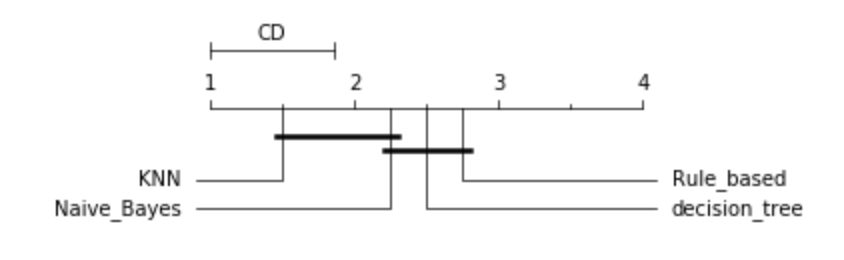
\includegraphics{CD.png}

We can see rule-based and K-nearest neighbor are most significantly different. In addition, decision tree and K-nearest neighbor are also significantly different.

\end{itemize}

\textbf{Conclusion:}
Different models for different datasets perform differently. Overall, for imbalanced dataset, after using sampling methods can improve the model performance. If the model could not work well after sampling, applying feature selection can improve the model performance in most cases. For testing different models significant difference, we can use Friedman test to analyze whether models are significantly different. If models are significantly different, then we use Nemenyi graph to analyze which pair of models are significantly different.

\end{document}
